\documentclass{report}

\usepackage[margin=1in]{geometry}
\usepackage{fancyhdr}
\usepackage{xr}
\usepackage{marginnote}
\usepackage{scrextend}
\usepackage[bottom]{footmisc}
\usepackage{enumitem}
\usepackage{amsmath,amssymb,amsthm}
\usepackage{bm}
\usepackage[hidelinks]{hyperref}

\fancypagestyle{main}{
    \fancyhf{}
    \fancyfoot[R]{Labalme\ \thepage}
    \fancyhead[R]{MATH\ 16210}
    \fancyhead[L]{\leftmark}
}
\fancypagestyle{plain}{
    \fancyhead{}
    \renewcommand{\headrulewidth}{0pt}
}

\externaldocument{main}
\externaldocument{../../../1 Autumn Quarter/Honors Calculus I IBL (Cartee)/MATH16110Notes/main}

\reversemarginpar

\deffootnotemark{\textsuperscript{\textup{[}\thefootnotemark\textup{]}}}
\deffootnote[2.1em]{0em}{0em}{\textsuperscript{\thefootnote}}

\newtheorem{theorem}{Theorem}[chapter]
\newtheorem{proposition}[theorem]{Proposition}
\newtheorem{lemma}[theorem]{Lemma}
\newtheorem{corollary}[theorem]{Corollary}
\theoremstyle{definition}
\newtheorem{definition}[theorem]{Definition}
\newtheorem{exercise}[theorem]{Exercise}
\newtheorem{remark}[theorem]{Remark}

\renewcommand{\chaptername}{Script}

\newcommand{\N}{\mathbb{N}}
\newcommand{\Z}{\mathbb{Z}}
\newcommand{\Q}{\mathbb{Q}}
\newcommand{\R}{\mathbb{R}}
\newcommand{\eqclass}[2]{\left[ \frac{#1}{#2} \right]}

\usepackage{subfiles}

\title{MATH 16210 (Honors Calculus II IBL) Notes}
\author{Steven Labalme}

\begin{document}




\maketitle



\pagenumbering{roman}
\tableofcontents
\newpage



\pagenumbering{arabic}
\pagestyle{main}
\renewcommand{\chaptermark}[1]{\markboth{\chaptername\ \thechapter}{}}
\setcounter{chapter}{5}
\subfile{Script06/script06.tex}


\section{Discussion}
\begin{itemize}
    \item \marginnote{1/12:}Upper limit at signing up for 4-5 across the script.
    \item Lemma \ref{lem:6.2} is probably more straightforward using a contradiction argument.
    \item Briefly restate the algebra of Exercise \ref{exr:4.24} in Exercise \ref{exr:6.3c}.
    \item \marginnote{1/14:}Turning in Script \ref{sct:5} journals is optional --- it will boost your grade a bit if you do.
    \begin{itemize}
        \item Your journal grade will be whichever is higher: the average of all your journal grades with and without Script \ref{sct:5}.
        \item Script \ref{sct:5} will probably be due Wednesday, 1/20.
    \end{itemize}
    \item In Lemma \ref{lem:6.6}, do we need to prove that the union of arbitrarily many Dedekind cuts is, itself, a Dedekind cut? Yes.
    \item \marginnote{1/18:}Is there a way to prove something else besides $A$ is not open in Exercise \ref{exr:6.7}?
    \begin{itemize}
        \item This is probably it as far as proving that continuua are connected.
        \item It may not be possible to prove that \emph{any} of the statements are wrong, but he's not sure.
    \end{itemize}
    \item Is Lemma \ref{lem:6.9} used in the proofs of any subsequent results, or is it just a less important result (hence the lemma designation)?
    \begin{itemize}
        \item We can think of it as an alternate definition for density --- we could prove Definition \ref{dfn:6.8} from it.
    \end{itemize}
    \item Is my handwavey use of Scripts \ref{sct:2} and \ref{sct:3} ok in Corollary \ref{cly:6.12}?
    \begin{itemize}
        \item I'm fine.
    \end{itemize}
    \item Is there a simpler way to prove Corollaries \ref{cly:6.12} and \ref{cly:6.14}?
    \begin{itemize}
        \item hi
    \end{itemize}
    \item Is the math REU still running this summer?
    \begin{itemize}
        \item He's not sure; UChicago's may not be NSF approved, hence why its not on the website rn.
    \end{itemize}
    \item What other summer opportunities would you recommend for a student at my level?
    \begin{itemize}
        \item He did an REU at UWisconsin when he was an undergrad.
        \item Sounds like its pretty much just REUs for undergrads.
        \item I could ask around to see if anyone is a Knot Theorist/willing to sponsor me.
    \end{itemize}
    \item \marginnote{1/19:}Easier Corollary \ref{cly:6.12}:
    \begin{itemize}
        \item Let $B>A$. Then $A<i(\frac{m}{q})<B$. Then $A<i(m)$.
    \end{itemize}
    \item Several proofs were given for Corollary \ref{cly:6.14}. One other correct one constructed the nonempty, bounded above set of all $i(n)$ less than or equal to $A$ and considered its supremum.
    \item \marginnote{1/21:}Now graded a bit more critically on presentations.
    \begin{itemize}
        \item Write big, talk loudly, don't talk to the blackboard.
    \end{itemize}
    \item My original proof of Corollary \ref{cly:6.14} is incorrect because I can't split into cases the way I did (\emph{longer expo}).
    \begin{itemize}
        \item Instead, use Seb's approach.
    \end{itemize}
    \item \marginnote{1/26:}Stray thoughts on Exercise \ref{exr:6.16}:
    \begin{itemize}
        \item Any property we can prove for $\Q$ (e.g., betweenness, Axioms 1-3, etc.) we should be able to prove for $K$.
        \begin{itemize}
            \item Many of these follow from $\Q$'s density! This is how we can make use of this condition.
        \end{itemize}
        \item We think of 0 as being somehow the "midpoint" of $\Q$. But since $\Q$ diverges in both directions, it doesn't really have a midpoint; we just assert this rather arbitrary structure on a more foundational algebraic construct.
        \begin{itemize}
            \item The same would hold for $K$. Thus, we can choose an arbitrary point $x\in K$ and let it be the "midpoint," i.e., let $f(0)=x$.
        \end{itemize}
        \item Can we induct on the elements of $\Q$? Since there exists a bijection $\Q\to\N$.
        \item We can construct an order preserving bijection between any finite subsets of $\Q$ and $K$ with equal cardinality.
        \item $f:\Q\to K$, $g:\N\to\Q$, $h:\N\to K$. If $g(n)<g(n')$, then $h(n)<h(n')$.
        \item Let $h(n)<h(n')$. WLOG let $n<n'$, too. Now consider $N=\{n\in\N\mid n\leq n'\}$. This is a finite set. Now create a new set $g(N)$. There will be an order-preserving bijection $\tilde{f}:h(N)\to g(N)$.
        \item Let $g:\N\to\Q$ be a bijection (we know one exists by countability). We presently seek to define $h:\N\to K$ recursively. Let $x_1$ be an arbitrary element of $K$ (Axiom 1). We define $h(1)=x_1$. Now suppose inductively that we have defined $h(n)$. We now seek to define $h(n+1)$. Consider the set $A=\{g(m)\mid m\leq n+1\}$. By Theorem \ref{trm:3.5}, we can assign the symbols $a_1,\dots,a_{n+1}$ to each point of $A$ so that $a_1<a_2<\cdots<a_{n+1}$. We know that $g(n+1)=a_i$ for some $i\in[n+1]$. We divide into three cases ($g(n+1)=b_1$, $g(n+1)=b_{n+1}$, and $g(n+1)=b_i$ where $1<i<n+1$). First, suppose that $g(n+1)=b_1$. By the inductive hypothesis, $h(g^{-1}(b_2))\in K$. By Axiom 3, $h(g^{-1}(b_2))$ is not the first point of $K$. Thus, there exists an $x\in K$ such that $x<h(g^{-1}(b_2))$. Consequently, let $h(n+1)=x$. The proof of the second case is symmetric to that of the first. Third, suppose that $g(n+1)=b_i$ where $1<i<n+1$. By the inductive hypothesis, $h(g^{-1}(b_{i-1})),h(g^{-1}(b_{i+1}))\in K$. Thus, there exists an $x\in K$ such that $h(b_{i-1})<x<h(b_{i+1})$. Consequently, let $h(n+1)=x$.
        \item We define $f:\Q\to K$ by $f(p)=h(g^{-1}(p))$.
        \item Function diagram: The characteristic of an order preserving bijection is no intersections between lines connecting elements of different sets.
    \end{itemize}
    \item Do we need to have subscripts on our orderings? Yes.
    \item The canonical way of doing Exercise \ref{exr:6.16} is with the \textbf{back and forth method}.
    \begin{itemize}
        \item Because both are countable, $\Q=\{q_1,q_2,\dots\}$. Likewise, $K=\{k_1,k_2,\dots\}$.
        \item To create the bijection, we have two repeating steps.
        \begin{enumerate}
            \item Let $i$ be the smallest index such that $q_i$ has not been paired.
            Let $j$ be an index such that $k_j$ hasn't been paired, and assigning $f(q_i)=k_j$ preserves ordering (we have to prove that such a $j$ exists). To prove this, we know that we can order the elements of $\Q$ that have already been paired. We can also order the elements of $K$ that have already been paired. Case 1: $q_i$ is between some preexisting $q$'s. Then there exists some $k_j$ between. Case 2: $q_i<\dots<q_n$ implies there exists some $k_j$ less than all other $k$ so far. Case 3: $q_i$ is a last element; symmetric to Case 2.
            \item Smallest $j$, smallest $i$ such that order is preserved. Then we let $f(q_i)=k_j$.
            \item Repeat.
        \end{enumerate}
        \item Injectivity: Suppose $f(q_i)=f(q_j)$. Each $q_k$ is assigned to a unique $k_k$, so if they're equal, they must have been assigned at the same time. Therefore, $q_i=q_j$.
        \item Surjectivity: Let $k_j\in K$. By $j$th step at most, $k_j$ will be paired.
    \end{itemize}
    \item Do summer research things every happen with graduate students, or is it just with professors? It pretty much only happens with professors, but DRP could be a good way to get your foot in the door.
\end{itemize}



\subfile{Script07/script07.tex}


\section{Discussion}
\begin{itemize}
    \item \marginnote{1/28:}Script 6 journals due Wednesday.
    \item We'll also have to prove a density lemma:
    \begin{itemize}
        \item Let $X$ be a dense subset of a continuum $C$. Show that for all $x,y\in X$, if $x<y$, then there exists a $z\in X$ such that $x<z<y$.
        \item Mark in Exercise \ref{exr:6.16} as "Density Lemma."
    \end{itemize}
    \item Explicitly cite Field Axioms as you go.
    \item \marginnote{2/2:}For Theorem 7.30 in class, he wants a simple explanation of what the injective map looks like and why, but not a full-on rigorous proof.
    \begin{itemize}
        \item Nothing in the journal for Theorem 7.30, though.
    \end{itemize}
    \item He also wants to see Exercises \ref{exr:7.32} and \ref{exr:7.40} in the journal.
    \item For Corollary \ref{cly:7.15}, we can write that $x^{-1}\cdot x=1$ and $x^{-1}\cdot(x^{-1})^{-1}=1$, and know by the uniqueness of multiplicative inverses (Theorem \ref{trm:7.14}) that $x=(x^{-1})^{-1}$. For Corollary \ref{cly:7.11}, we have an analogous proof.
    \item Alternate Theorem \ref{trm:7.17}:
    \begin{align*}
        1 &= 1\cdot 1\\
        &= (a\cdot a^{-1})(b\cdot b^{-1})\\
        &= (ab)(a^{-1}b^{-1})\\
        &= 0
    \end{align*}
    \item Alternate Lemma \ref{lem:7.18}: $a+(-a)=0$. $a+(-1)a=a(1+(-1))=a\cdot 0=0$. Thus, by Theorem \ref{trm:7.10}, $-a=(-1)a$.
    \item Alternate Lemma \ref{lem:7.19}: We can use the uniqueness of additive inverses (Theorem \ref{trm:7.10}).
    \item We can also cite Remark \ref{rmk:7.25} in Lemma \ref{lem:7.26}.
    \item \marginnote{2/4:}Thoughts on Theorem 7.30:
    \begin{figure}[h!]
        \centering
        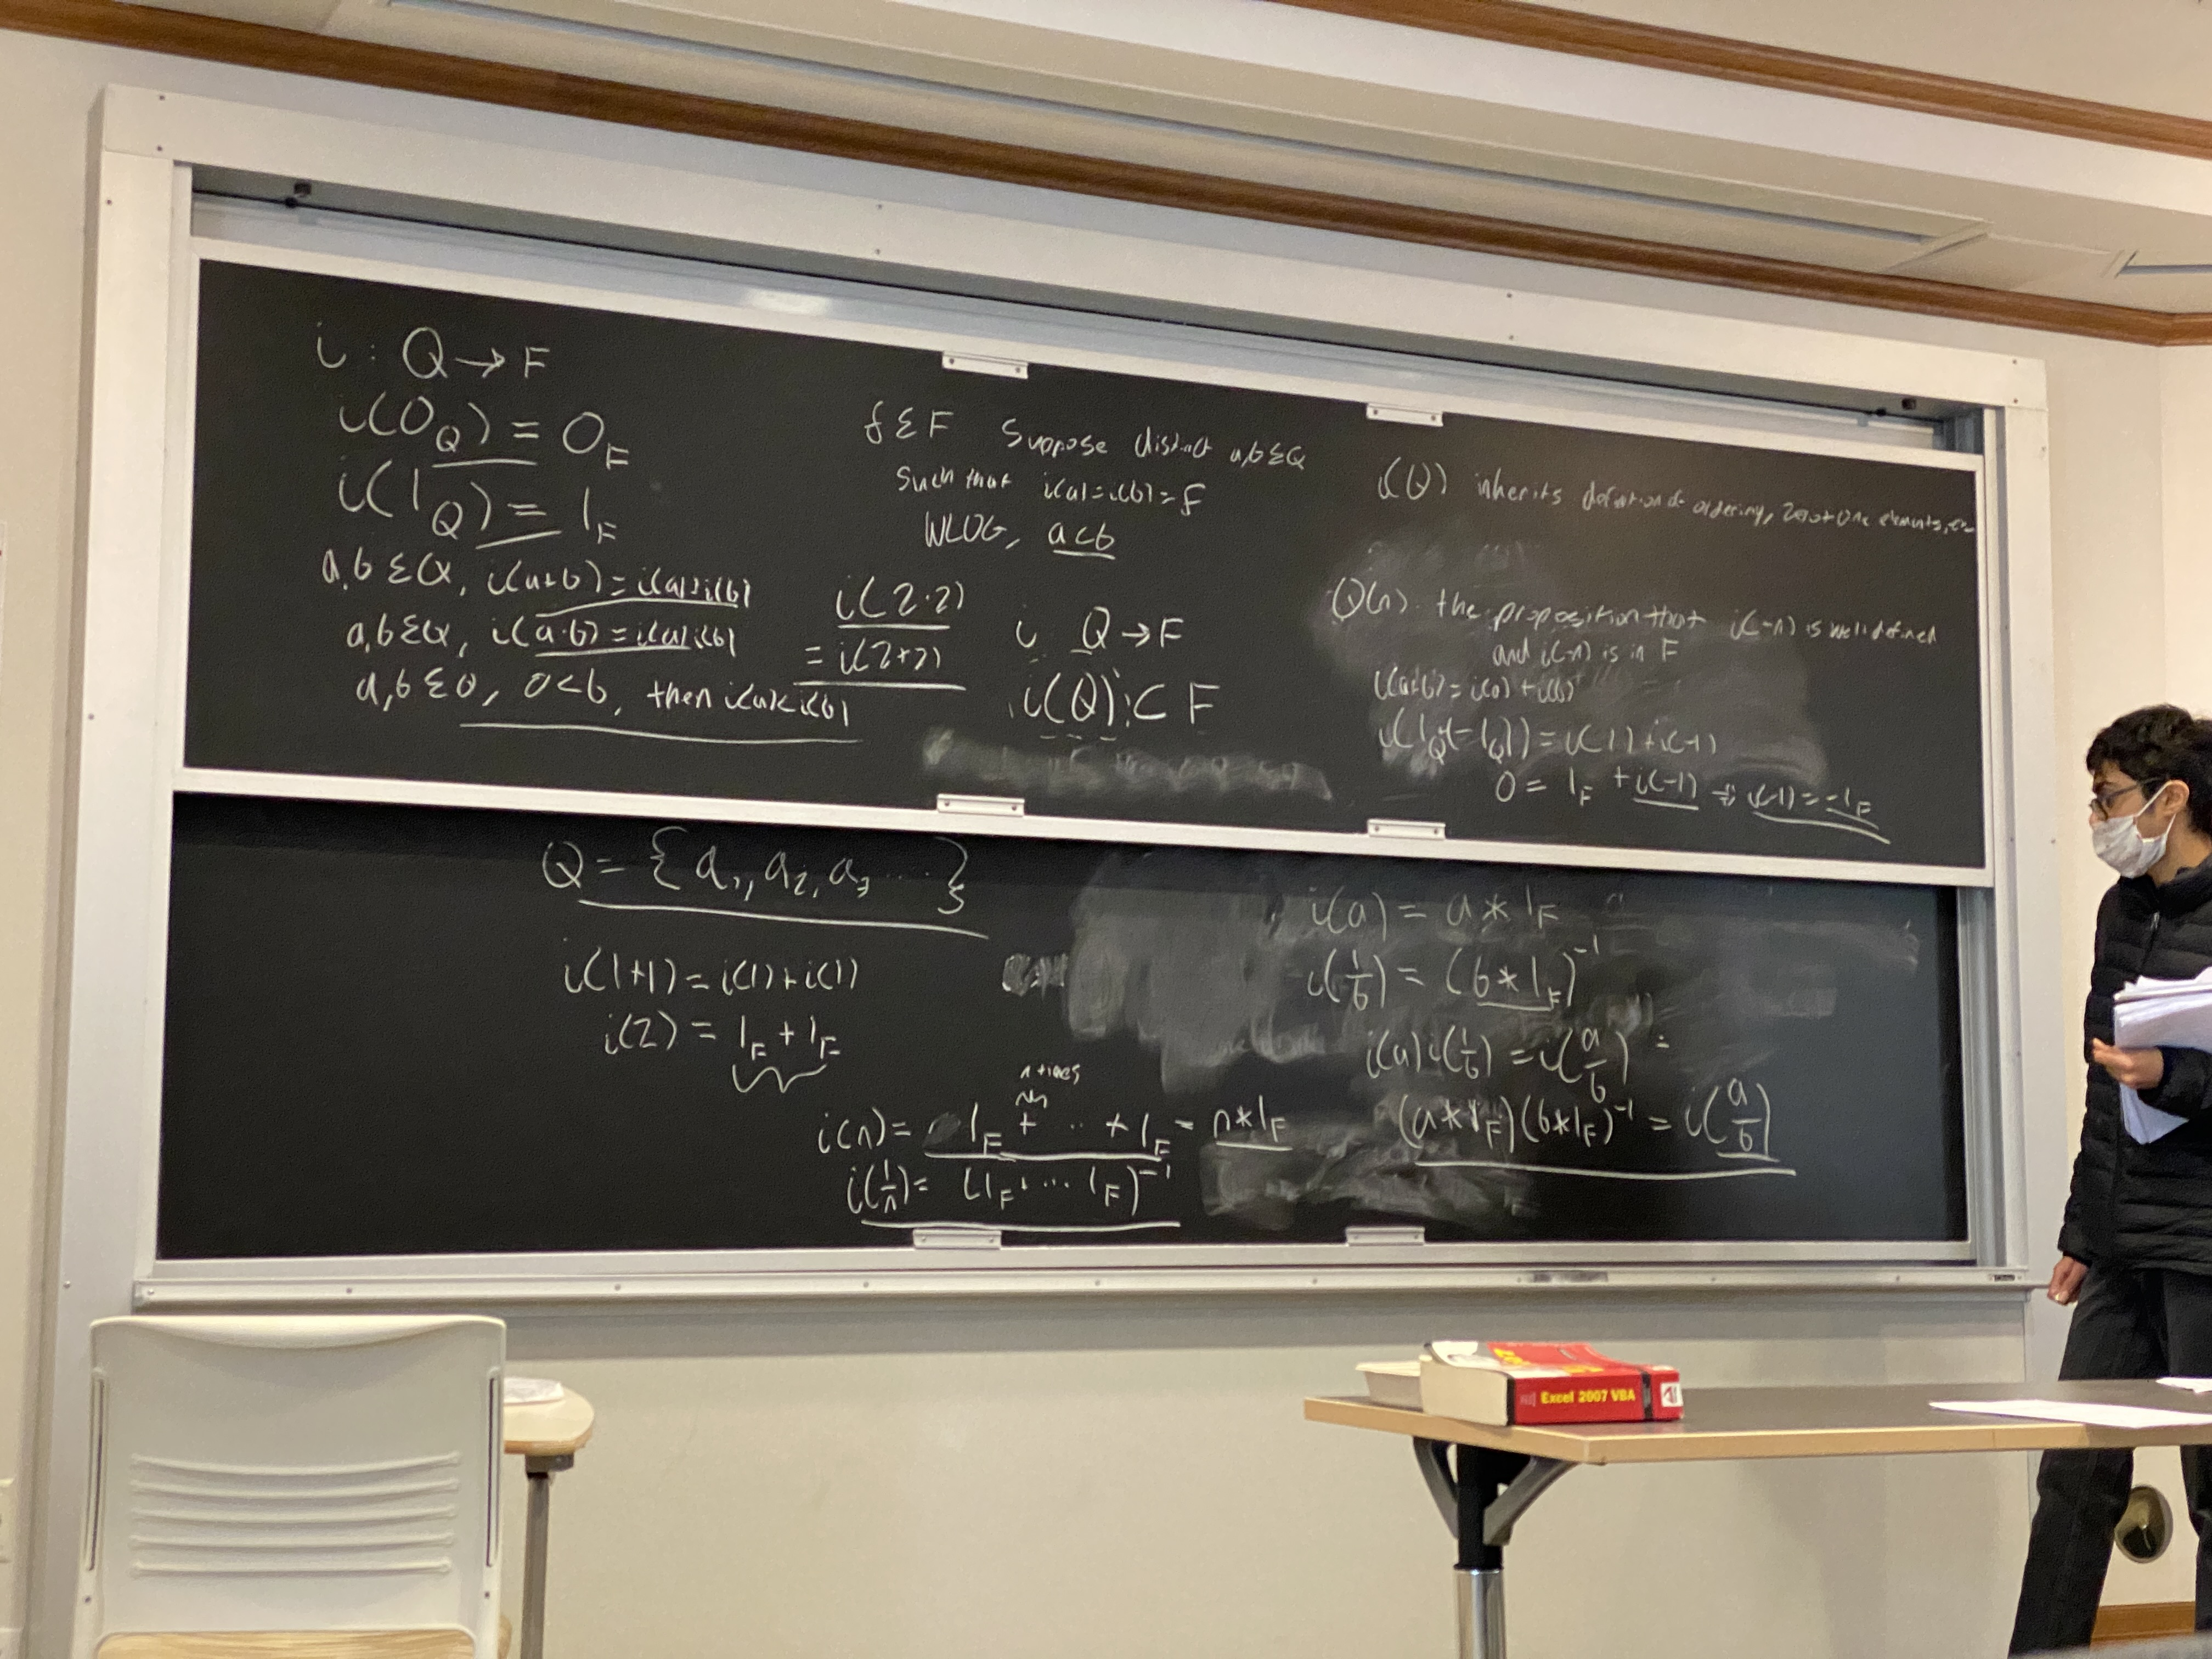
\includegraphics[width=0.5\linewidth]{ExtFiles/theorem7-30.JPG}
        \caption{Theorem 7.30 discussion.}
        \label{fig:theorem7-30}
    \end{figure}
\end{itemize}



\subfile{Script08/script08.tex}


\section{Discussion}
\begin{itemize}
    \item \marginnote{2/9:}Due date: Feb. 19; if there's anything I can provide that would facilitate the process, lmk; Know anything about mixed-integer nonlinear programming?
    \item Lemma \ref{lem:8.3} more efficiently by proving that every $x\in(a,b)$ is an element of $I$ and then just working with the boundary conditions?
    \begin{itemize}
        \item Make first four cases of second direction symmetric.
    \end{itemize}
    \item Rewrite Exercise \ref{exr:8.5} with three cases: $x=0$, $x>0$, $x<0$ with the last two symmetric.
    \item We don't have to cite every algebraic manipulations from Script \ref{sct:7}.
    \item \marginnote{2/11:}Use a bidirectional inclusion proof instead of set algebra for Exercise \ref{exr:8.13}.
    \item What is the problem with Exercise \ref{exr:8.14b}?
\end{itemize}



\subfile{Script09/script09.tex}


\section{Discussion}
\begin{itemize}
    \item \marginnote{2/16:}For Proposition \ref{prp:9.5}, do an iff proof --- use $\Longleftrightarrow$ steps instead of back-and-forth work.
    \item \marginnote{2/18:}To what extent do we need casework in Theorem \ref{trm:9.14}?
\end{itemize}



\subfile{Script10/script10.tex}


\section{Discussion}
\begin{itemize}
    \item \marginnote{2/25:}Script \ref{sct:9} journals due next Wednesday.
    \item \marginnote{3/2:}$(a,b)$ is not closed, compact, so I have to change my answer to no for the question associated with Theorem \ref{trm:10.15}.
    \begin{itemize}
        \item Also show this as a lemma.
    \end{itemize}
    \item For Lemma \ref{lem:10.13}, $s'$ is a better variable name than $y$.
    \item For Theorem \ref{trm:10.14}, I don't need casework --- if we negate $x_{i-1}<y\leq x_i$, we have $y<x_0$ or $y>x_n$, contradictions in either way, so straight-up suppose it.
    \item Dramatically simplify Theorem \ref{trm:10.15} with $\mathcal{G}\cup(\R\setminus Y)$ as a cover of $X$ where $\mathcal{G}$ is an arbitrary open cover of $Y$.
    \item FSC as an abbreviation for \underline{F}or the \underline{S}ake of \underline{C}ontradiction.
    \item Simplify Theorem \ref{trm:10.18} by supposing $X$ has no limit points, noting that this implies it's closed. It follows that it's compact and that it's finite, a contradiction.
    \item Is it true that a set is compact iff it is the union of finitely many closed intervals?
\end{itemize}




\end{document}